\documentclass{article}
\usepackage{graphicx}
\usepackage{amsmath}
\usepackage{amssymb}
\usepackage{natbib}
\renewcommand{\refname}{References}
\usepackage{url}

\title{A Differential Geometric Approach to Economic Forecast}

\author{Babak Emami}

\date{\today}

\begin{document}
\maketitle

\begin{abstract}


\end{abstract}

\section{Introduction}\label{section:introduction}

The usual approach to predicting price of an asset is to regress the
historical prices of tat asset against a set of economic
indicators. The problem with this approach is that we still need
knowldege of the future values of economic indicators. This is done by
relying on estimate forecasts of econimic indicators which are often
based on qualitative methods, such as those in Blue Chip Economic
Indicators and Blue Chip Financial Forecasts~\cite{ref:blue-chip}. The
forecasts in Blue Chip publications are based on surveying top
business economists in the United States.

An approach is proposed to forecast economic variables without
depending on future values of any economic indicators. We look at the
economy as a multi-demensional manifold; each dimension is an economic
variable. These variables can be marco-economic indicators or asset
prices. We refer to this manifold as an economic universe. The
observed values of economic variables in a time period form a path in
this universe. We refer to this path as the economic path. We then
find a manifold for which this path is a geodesic, governed by a
system of differential equations. The fututre value of economc
variables can be predicted by solving this system of differential
equations.

In what follows the mathematical framework used is discussed and a
methodology is proposed to infer the structure of economic universe
given a set of observed economic variables. Some results are presented
followed by a model parameter study. Finally, a trading algorithm is
proposed using this approach to forecast asset prices.

\section{Mathematical Framework}\label{section:mathematical-framework}

Let us consider $n$ variables $x{1}$ to $x^{n}$ that are smooth
functions of time $t$; $x^{i} = x^{i}(t)$. Moreover, let us consider a
smooth real manifold $M$ equipped with $(x^{1},x^{2},...,x^{n})$ as a
coordinate system. Each set of coordinate values
$(x^{1}(t),...,x^{n}(t))$ denotes a point $p$ on $M$. Values of these
$n$ variables over a period of time $[0,T]$ form a path over $M$. This
path is smooth as $x^{i}$s are smooth functions of time. Now let us
add a constraint on $M$ by assuming that the path formed by
$x^{i}(t)$s is a geodesic of $M$. With this assumption, this path is
governed by the follwoing system of ordinary differential equations,

\begin{equation}\label{eqn:geodesic}
\ddot{x}^{m} + \Gamma^{m}_{ab} \dot{x}^{a} \dot{x}^{b} = 0
\end{equation}

The Christoffel symbols $Gamma^{m}_{ab}$ are in general functions of
coordinates. In the current work, we assume that Christoffel symbols
are constant. This is a sufficient (but not necessary) condition for
the manifold to have a constant curvature. This assumption is rather
strong and as such we should revisit this subject.

To further simplify the problem, we assume that variables of interest
are in fact $y^{m} = \frac{dx^{m}}{dt}$. This will allow us to work
with a set of first order ODEs,

\begin{equation}\label{eqn:geodesic-1st-order}
\dot{y}^{m} + \Gamma^{m}_{ab} y^{a} y^{b} = 0
\end{equation}

The above system of ODEs needs a boundary condition,

\begin{equation}\label{eqn:geodesic-bc}
\dot{y}^{m}(t_{BC}) = \dot{y}^{m}_{0}
\end{equation}

where $m,a,b \in [1,n] \cap \mathbb{N}$, and $t_{BC}$ is the time at
which a boundary condition is set.

This means that the variables of interest are elements of the tangent
bundle of manifold $M$, that is $y^{m}(t) \in T_{p(t)}M$, where $p(t)
\in M$ corresponds to coordinates $(x^{1},x^{2},...,x^{n})$.

Now, let us further assume that the values of variables $y^{m}(t)$ are
known for $t \in [0,T]$. Using this a set of training data, we can
determine $Gamma^{m}_{ab}$ by fitting Eq.~\ref{eqn:geodesic-1st-order}
over the training data. This can be done using a continuous adjoint
approach.

\section{Some Results}\label{section:results}

A 33-dimensional manifold is built using the above-mentioned
approach. The dimensions of the manifold correspond to prices of the
following ETFs (exchanged-traded funds),

    QQQ: PowerShares QQQ
    SPY: SPDR S&P 500 Growth ETF
    DIA: SPDR Dow Jones Industrial Average ETF
    MDY: SPDR S&P MidCap 400 ETF
    IWM: iShares Russell 2000 Index Fund
    OIH: Market Vectors Oil Services ETF
    SMH: Market Vectors Semiconductor ETF
    XLE: Energy Select Sector SPDR Fund
    XLF: Financial Select Sector SPDR Fund
    XLU: Utilities Select Sector SPDR Fund
    EWJ: iShares MSCI Japan Index Fund

prices of the following (continuous) futures contracts,

    ES: E-mini S&P 500 Continuous Contract
    NQ: E-mini Nasdaq 100 Continuous Contract
    YM: E-mini Dow Futures Continuous Contract
    RTY: E-mini Russell 2000 Continuous Contract
    EMD: E-mini S&P MidCap 400 Continuous Contract
    QM: E-mini Crude Oil Futures Continuous Contract
    US: 30 Year U.S. Treasury Bonds Continuous Contract    

and values of the following financial indices,

    INDU: Dow Jones Industrial Average
    NDX: Nasdaq 100 Index
    SPX: S&P 500 Index
    COMPX: Nasdaq Composite Index
    RUT: Russell 2000 Index
    OEX: S&P 100 Index
    MID: S&P 400 Midcap Index
    SOX: PHLX Semiconductor Sector Index
    RUI: Russell 1000 Index
    RUA: Russell 3000 Index
    TRAN: Dow Jones Transportation Average
    HGX: PHLX Housing Sector Index
    TYX: 30-Year Treasury Bond
    HUI: NYSE Arca Gold BUGS Index
    XAU: PHLX Gold/Silver Sector Index

Here we assume that the above variables are elements of the tanget
bundle of our manifold, that is $y^{m}(t)$ in
Eq.~\ref{eqn:geodesic-1st-order}. In other words, coordinates of our
manifold, $x^{m}(t)$ in Eq.~\ref{eqn:geodesic}, are cumulative of the
above variables.

We trained this maniofold using intraday minute-based data spanning
2017-01-03 to 2018-01-03. The model is tested on three days of
out-of-sample data corresponding to the first three business days
after training period. Figure~\ref{fig:results-spy} shows in-sample
and out-of-sample forecast results for SPY as a function of time in
minutes; figure~\ref{fig:results-spy-oos} is zoomed on the
out-of-sample forecast. The out of sample results are reasonable. The
average relative error of out-of-sample forecasts of all variables in
the model is 3.5\%.

\begin{figure}\label{fig:results-spy}
\includegraphics[bb=0 0 640 480]{figures/results-SPY.png}
\caption{In-sample and out-of-sample forecast results for SPY.}
\end{figure}

\begin{figure}\label{fig:results-spy-oos}
\includegraphics[bb=0 0 640 480]{figures/results-SPY-oos.png}
\caption{Out-of-sample forecast results for SPY.}
\end{figure}

\section{Model Parameter Study}\label{section:model-parameter-study}

\begin{figure}\label{fig:tolerance-sensitivity-error}
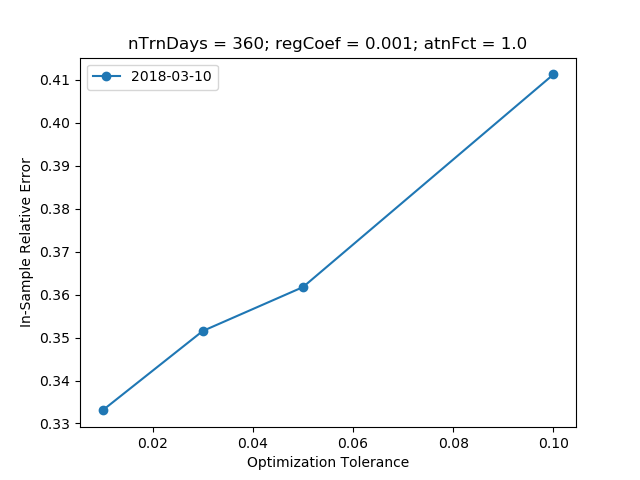
\includegraphics[bb=0 0 640 480]{figures/tolerance-sensitivity-error.png}
\caption{In-sample relative error vs. optimization tolerance.}
\end{figure}

\begin{figure}\label{fig:tolerance-sensitivity-oos-error}
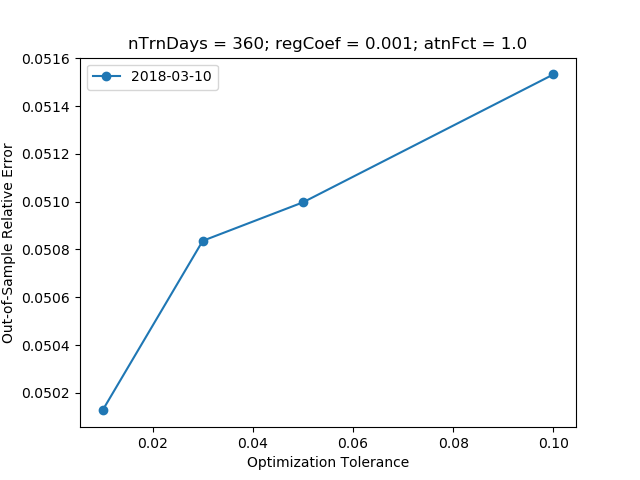
\includegraphics[bb=0 0 640 480]{figures/tolerance-sensitivity-oos-error.png}
\caption{Out-of-sample relative error vs. optimization tolerance.}
\end{figure}

\begin{figure}\label{fig:nTrnDays-sensitivity-error}
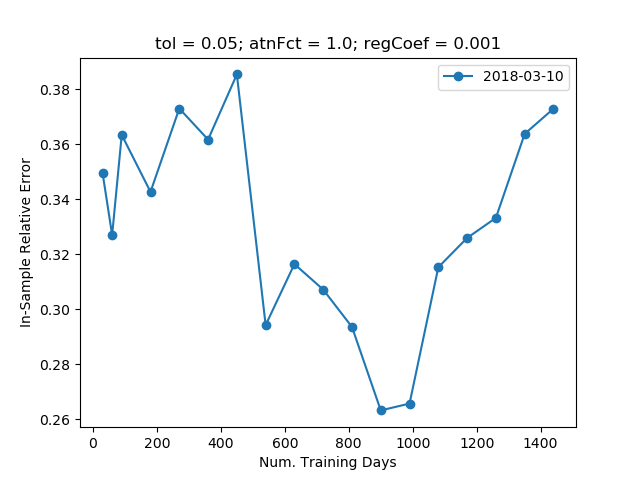
\includegraphics[bb=0 0 640 480]{figures/nTrnDays-sensitivity-error.png}
\caption{In-sample relative error vs. number of days used for training.}
\end{figure}

\begin{figure}\label{fig:nTrnDays-sensitivity-oos-error}
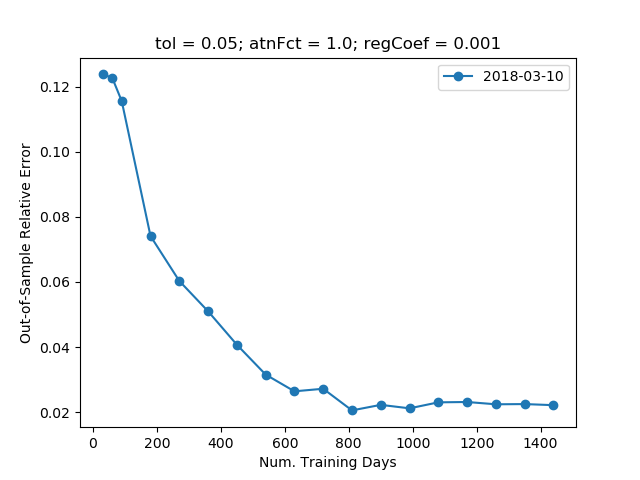
\includegraphics[bb=0 0 640 480]{figures/nTrnDays-sensitivity-oos-error.png}
\caption{Out-of-sample relative error vs. number of days used for training.}
\end{figure}

\begin{figure}\label{fig:regCoef-sensitivity-error}
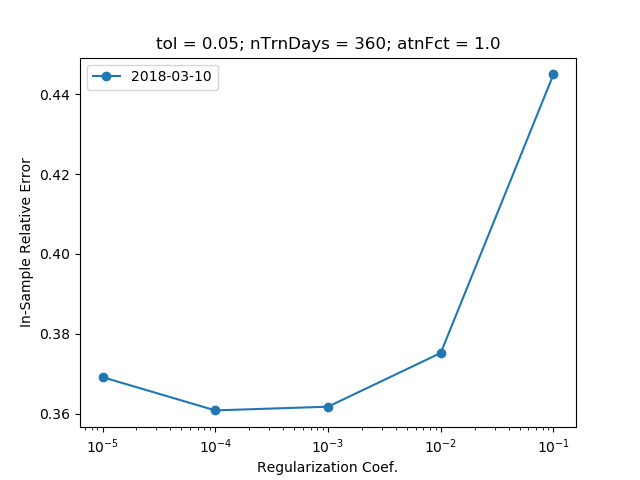
\includegraphics[bb=0 0 640 480]{figures/regCoef-sensitivity-error.png}
\caption{In-sample relative error vs. regularization coefficient.}
\end{figure}

\begin{figure}\label{fig:regCoef-sensitivity-oos-error}
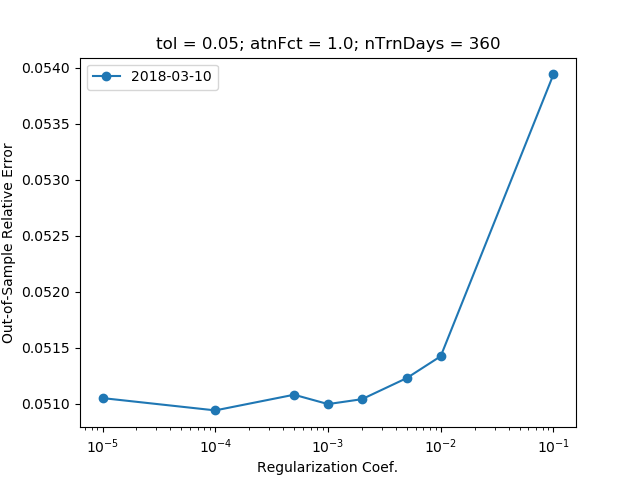
\includegraphics[bb=0 0 640 480]{figures/regCoef-sensitivity-oos-error.png}
\caption{Out-of-sample relative error vs. regularization coefficient.}
\end{figure}

\begin{figure}\label{fig:atnFct-sensitivity-error}
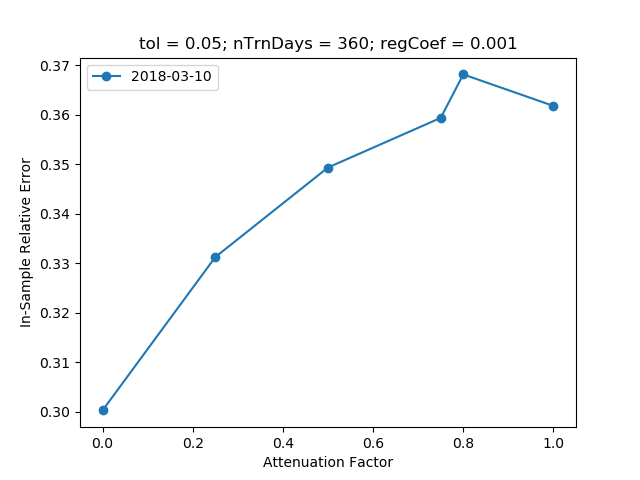
\includegraphics[bb=0 0 640 480]{figures/atnFct-sensitivity-error.png}
\caption{In-sample relative error vs. attenuation coefficient.}
\end{figure}

\begin{figure}\label{fig:atnFct-sensitivity-oos-error}
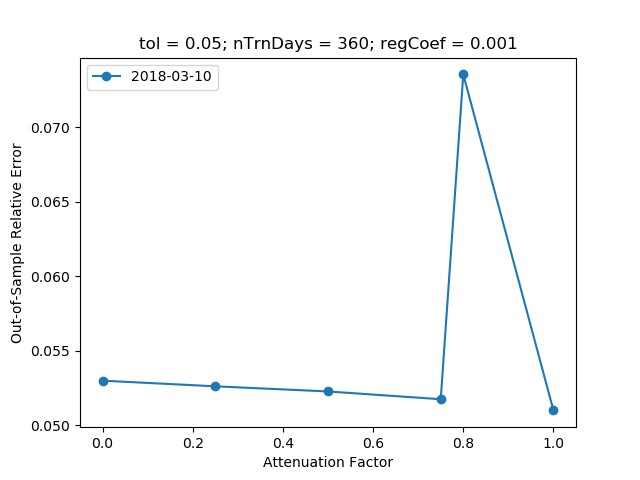
\includegraphics[bb=0 0 640 480]{figures/atnFct-sensitivity-oos-error.png}
\caption{Out-of-sample relative error vs. attenuation coefficient.}
\end{figure}

\section{On Behavior of Christoffel Symbls}\label{section:christoffel-behavior}

\begin{figure}\label{fig:gamma-time}
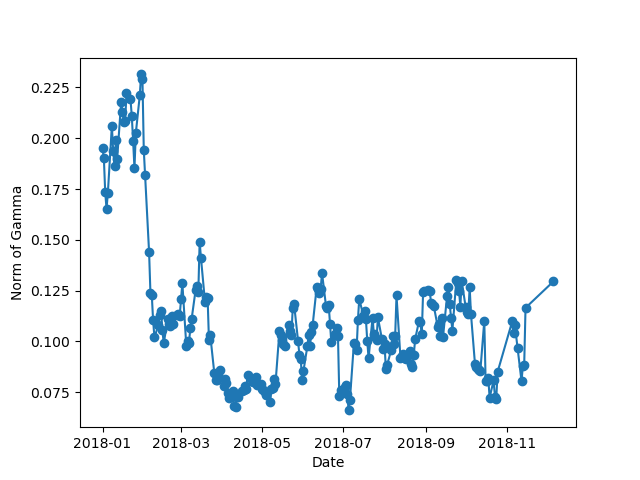
\includegraphics[bb=0 0 640 480]{figures/Gamma_time_2018.png}
\caption{Norm of Gamma vs. snapdate Each point on the plot comes from
  a model with a constant Christoffel symbol.}
\end{figure}

\section{A Proposed Trading Algorithm}\label{section:trading-algorithm}

\section{Conclusions}\label{section:conclusions}

\bibliography{references}
\bibliographystyle{plain}

\end{document}

